\documentclass[a4paper,12pt]{article}
\usepackage[utf8]{inputenc}
\usepackage[spanish]{babel}
\usepackage{graphicx}
\usepackage{libertine}
\usepackage{amsmath}
\renewcommand\familydefault{\sfdefault}
\usepackage[T1]{fontenc}
\usepackage[colorlinks=true,linkcolor=blue]{hyperref}
\usepackage[framed,numbered,autolinebreaks,useliterate]{mcode}

\parindent = 0mm

\author{Moisés Gautier Gómez}
\title{
\includegraphics[width=10cm]{logo_ugr.png} \\ 
\includegraphics[width=3cm]{fetch.png}\\ Práctica 4 - Teoría de la Señal y Comunicaciones 
}
\date{ }

\begin{document}
\maketitle
Ejercicios
%\lstinputlisting{genexp.m}

\begin{enumerate}
\item Obtenga la expresión matemática de cada una de las ventanas especificadas anteriormente y
represente el modulo en dB de las mismas. \\

Para las representaciones gráficas he utilizado un tamaño de ventana de 40, y para el desarrollo de las expresiones matemáticas un tamaño $N$, donde $0 \leq n \leq N -1$.

\begin{itemize}
\item Ventana Rectangular.
$$v(n) = 1$$
\hspace*{-1.5in}{
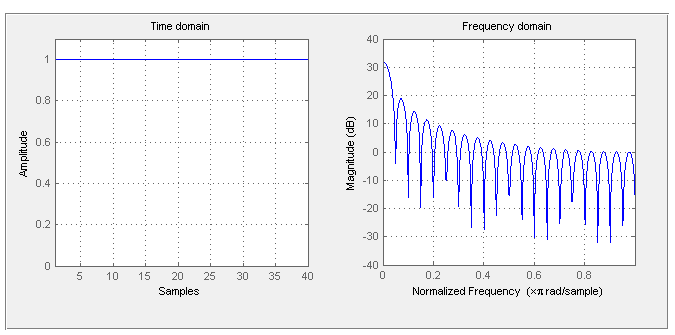
\includegraphics{ej1-1-rectangular.png}
}
\item Ventana Bartlett.
$$v(n) = \frac{N-1}{2} - \bigg|n - \frac{N-1}{2} \bigg|$$
\hspace*{-1.5in}{
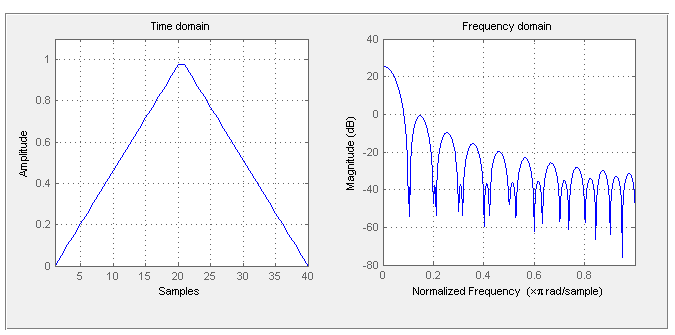
\includegraphics{ej1-2-bartlett.png}
}
\item Ventana Hamming.
$$v(n) = a_0 - a_1 \cos(\frac{2 \pi n}{N -1})$$
$$ a_0 = 0,53836;\ a_1 = 0,46164;\ $$
\hspace*{-1.5in}{
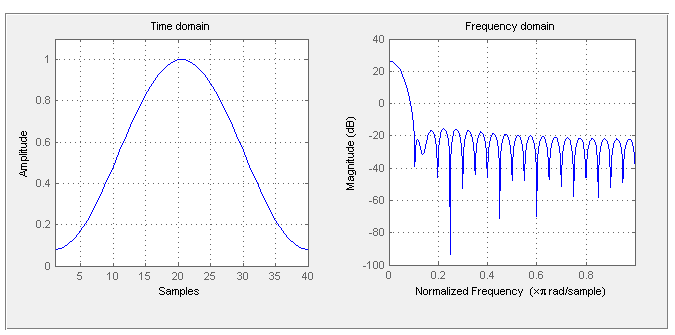
\includegraphics{ej1-3-hamming.png}
}
\item Ventana Hanning.
$$v(n) = a_0 - a_1 \cos(\frac{2 \pi n}{N -1})$$
$$ a_0 = 0,5;\ a_1 = 0,5;\ $$
\hspace*{-1.5in}{
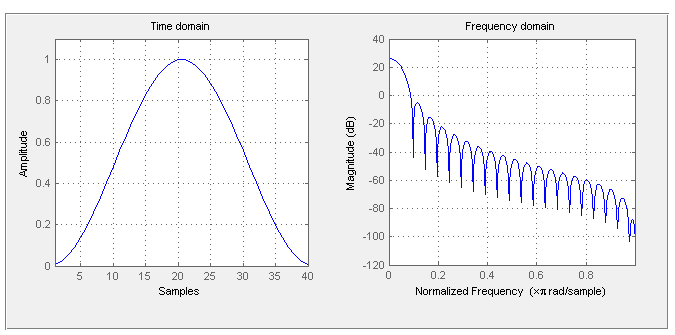
\includegraphics{ej1-4-hanning.png}
}
\item Ventana Blackman.
$$v(n) = a_0 - a_1 \cos(\frac{2 \pi n}{N -1}) + a_2 \cos(\frac{4 \pi n}{N -1})$$
$$ a_0 = 0,42;\ a_1 = 0,5;\ a_2 = 0,08;\ $$
\hspace*{-1.5in}{
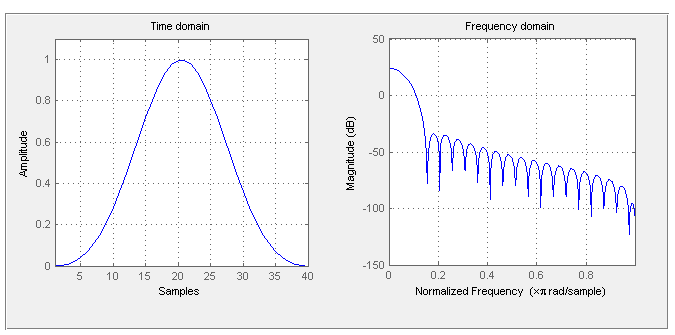
\includegraphics{ej1-5-blackman.png}
}
\item Ventana Kaiser.
Empleo un valor de 5 para el parámetro Beta de la ventana Kaiser. \\
\[ w_k = \left\{ 
  \begin{array}{l l}
    \frac{I_0 \bigg(\pi \beta \sqrt{1 - \bigg( \frac{2^K}{n -1} \bigg)^2} \bigg)}{I_0 (\pi \beta)} & \quad \text{si } 0 \leq k \leq n \\
    0 & \quad \text{resto}
  \end{array} \right.\]
\hspace*{-1.5in}{
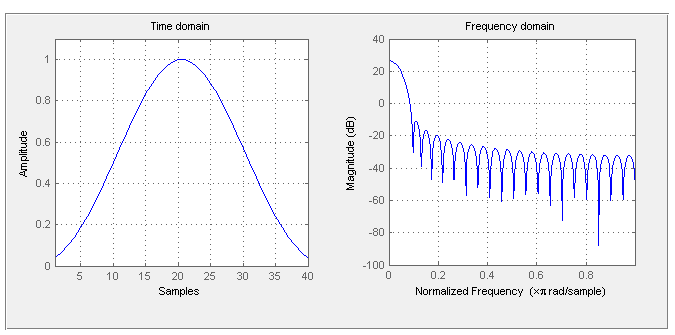
\includegraphics{ej1-6-kaiser.png}
}
\end{itemize}

Ahora voy a incluir el código que he generado para este ejercicio en matlab: \\
\lstinputlisting{Ejercicio-1.m}

\item Determine la anchura del lóbulo central de los siguientes tipos de ventanas: rectangular, Bartlett, de Hamming y de Blackman, de longitud 31 puntos. Tome como referencia el ancho a 3dB. Verifique también la altura del primer lóbulo lateral. \\
\begin{itemize}
\item Ventana Rectangular:\\
\hspace*{-1.5in}{
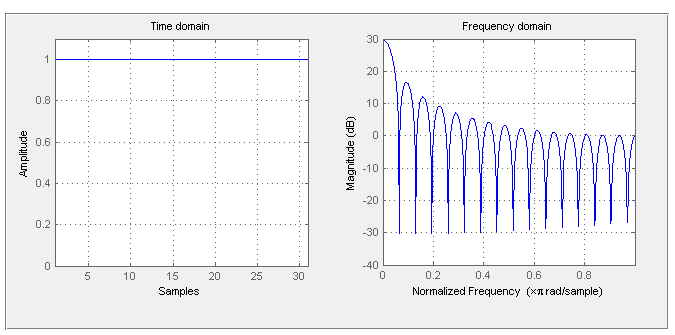
\includegraphics{ej2-1-rectangular.png}
}\\
Anchura del principal: 0,054688; Atenuación: -13,3 dB; Altura del primer lateral: 15 dB.
\item Ventana Bartlett:\\
\hspace*{-1.5in}{
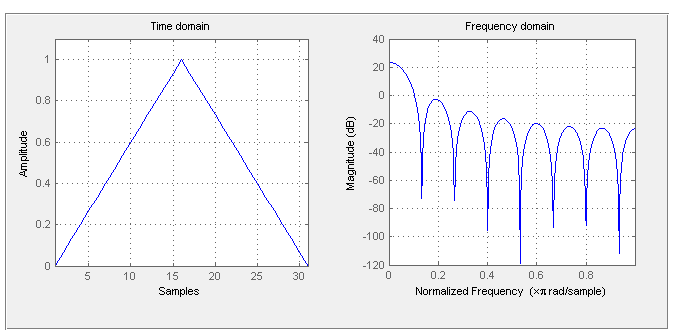
\includegraphics{ej2-2-bartlett.png}
}\\
Anchura del principal: 0,078125; Atenuación: -26,3 dB; Altura del primer lateral: 0 dB.
\item Ventana Hamming:\\
\hspace*{-1.5in}{
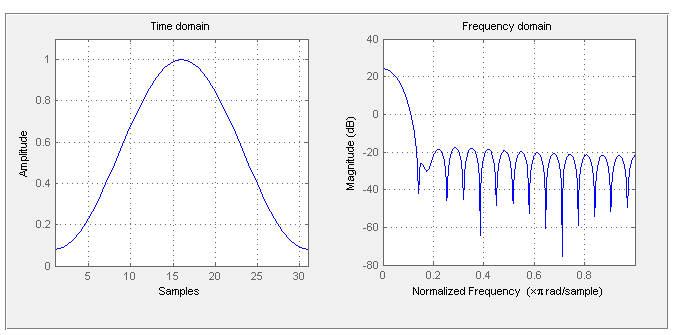
\includegraphics{ej2-3-hamming.png}
}\\
Anchura del principal: 0,078125; Atenuación: -41,7 dB; Altura del primer lateral: -20 dB.
\item Ventana Blackman:\\
\hspace*{-1.5in}{
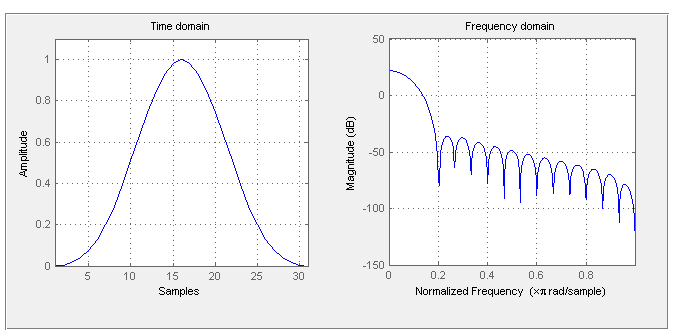
\includegraphics{ej2-4-blackman.png}
}\\
Anchura del principal: 0,10938; Atenuación: -58,2 dB; Altura del primer lateral: -30 dB.
\end{itemize}

Ahora voy a incluir el código que he generado para este ejercicio en matlab: \\

\lstinputlisting{Ejercicio-2.m}
\item Para cada una de las ventanas definidas en el apartado anterior verifique el efecto de incrementar la longitud de la ventana tanto en el lóbulo central como en los lóbulos laterales. \\

Compararemos dos tamaños de ventana, 40 (la gráfica en color azul) y 80 (la gráfica en color verde).\\

\begin{itemize}
\item Ventana Rectangular:\\
\hspace*{-1.5in}{
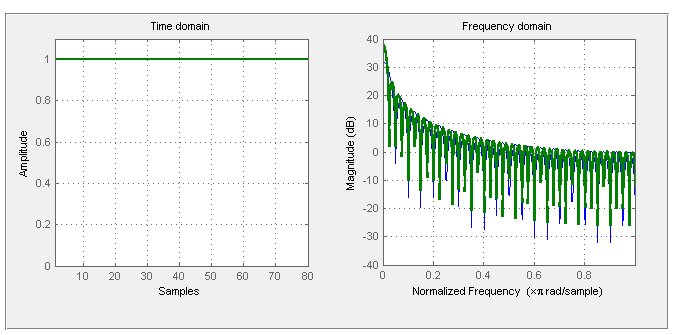
\includegraphics{ej3-1-rectangular.png}}
\item Ventana Bartlett: \\
\hspace*{-1.5in}{
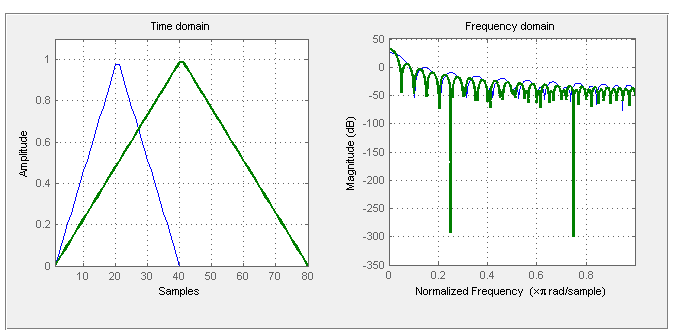
\includegraphics{ej3-2-bartlett.png}}
\item Ventana Hamming: \\
\hspace*{-1.5in}{
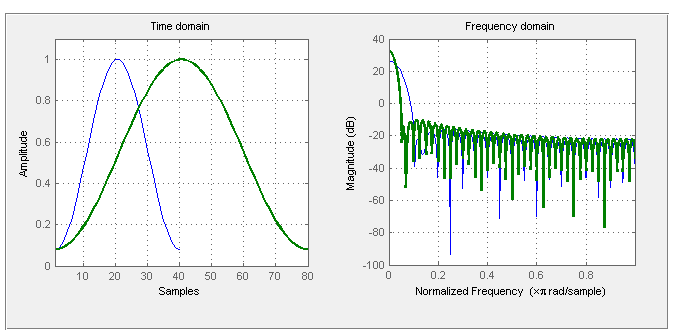
\includegraphics{ej3-3-hamming.png}}
\item Ventana Blackman: \\
\hspace*{-1.5in}{
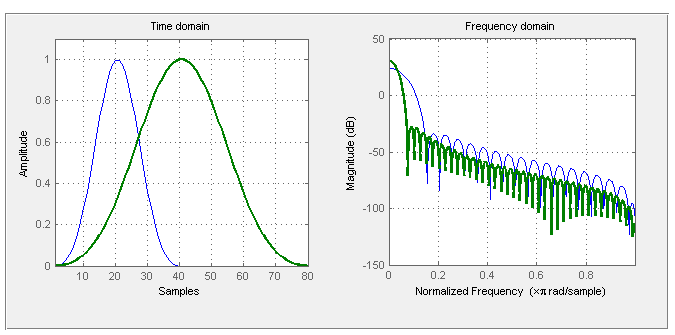
\includegraphics{ej3-4-blackman.png}}
\end{itemize}

Podemos observar en las siguiente gráficas como al aumentar el tamaño de la ventana al doble, la anchura del lóbulo principal se reduce a la mitad, mientras que la altura de los lóbulos laterales permanece inalterable en el tiempo. \\

Ahora voy a incluir el código que he generado para este ejercicio en matlab: \\

\lstinputlisting{Ejercicio-3.m}

\item Estudie el comportamiento de los lóbulos laterales para una ventana de Kaiser en función del parámetro $\beta$. Para ello genere 3 ventanas de Kaiser de longitud 31 y $\beta$ = 3, 5 y 8. Estudie la relación entre la altura de los lóbulos laterales y la anchura del lóbulo principal. \\

\begin{itemize}
\item $\beta = 3$:\\
\hspace*{-1.5in}{
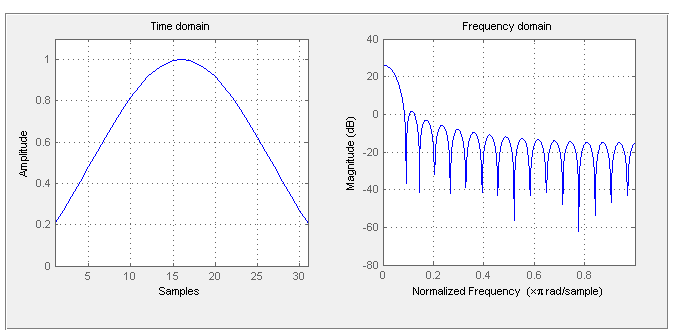
\includegraphics{ej4-1-kaiser.png}}
\item $\beta = 5$:\\
\hspace*{-1.5in}{
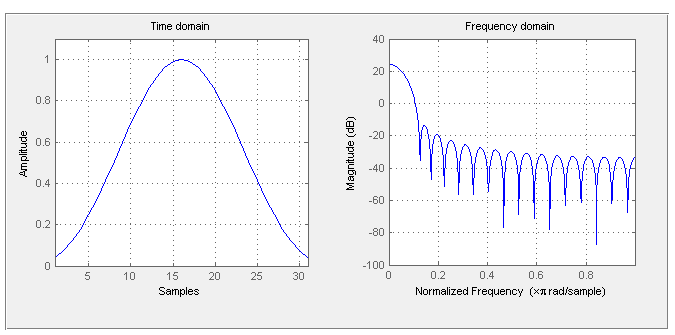
\includegraphics{ej4-2-kaiser.png}}
\item $\beta = 8$:\\
\hspace*{-1.5in}{
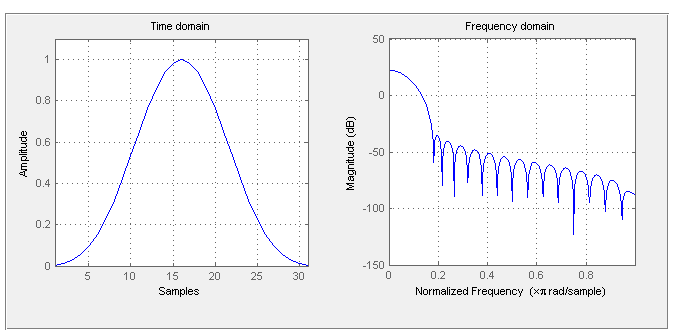
\includegraphics{ej4-3-kaiser.png}}
\end{itemize}

Al aumentar $\beta$, se estrecha más nuestra ventana, por lo que aumenta la anchura del lóbulo principal y disminuye la altura (amplitud) de los lóbulos laterales. \\

Ahora voy a incluir el código que he generado para este ejercicio en matlab: \\

\lstinputlisting{Ejercicio-4.m}

\item Encuentre en internet documentación relativa al análisis de Fourier de tiempo corto (STFT) y
estúdiela en detalle. \\

Dentro de una gran variedad de artículos y enlaces web he seleccionado los siguiente como más importantes:
\begin{itemize}
\item \href{http://en.wikipedia.org/wiki/Short-time_Fourier_transform}{STFT wikipedia inglesa}
\item \href{http://www.mathworks.com/matlabcentral/fileexchange/38773-short-time-fourier-transform}{Ejemplo en Matlab} 
\item \href{https://www.math.ucdavis.edu/~strohmer/research/gabor/gaborintro/node3.html}{Local time-frequency analysis and short time Fourier transform}
\end{itemize}

\item Cargue en matlab la señal de voz signal.asc (muestreada a 8kHz) y utilice la función specgram de Matlab para representar el espectrograma. Utilice una ventana de Hamming longitud 20ms. Observe la evolución de las trayectorias de los formantes. \\

Voy a mostrar directamente la ejecución que realizo en matlab y posteriormente la imagen resultado que nos devuelve el software: \\

\lstinputlisting{Ejercicio-6.m}
\hspace*{-.75in}{
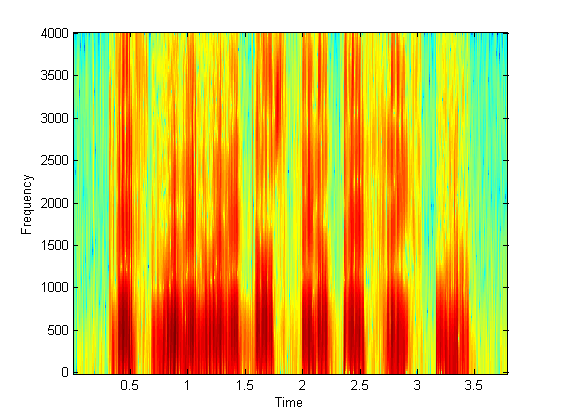
\includegraphics{ej6-espectograma.png}}

\item Implemente en Matlab su propia función \textbf{specgram}. Esta función deberá de admitir que el usuario determine al menos el tamaño de la ventana de análisis y el tipo de ventana a elegir entre ventana de Hamming , de Bartlett o rectangular. \\

Yo para este ejercicio, en vez de implementar una función que simule el comportamiento de \textbf{specgram} directamente, he implementado una gui que ofrece matlab en donde el usuario pueda interactuar de una manera más sencilla y dinámica. \\

Pongo algunos ejemplos realizados con la interfaz:\\
\hspace*{-.75in}{
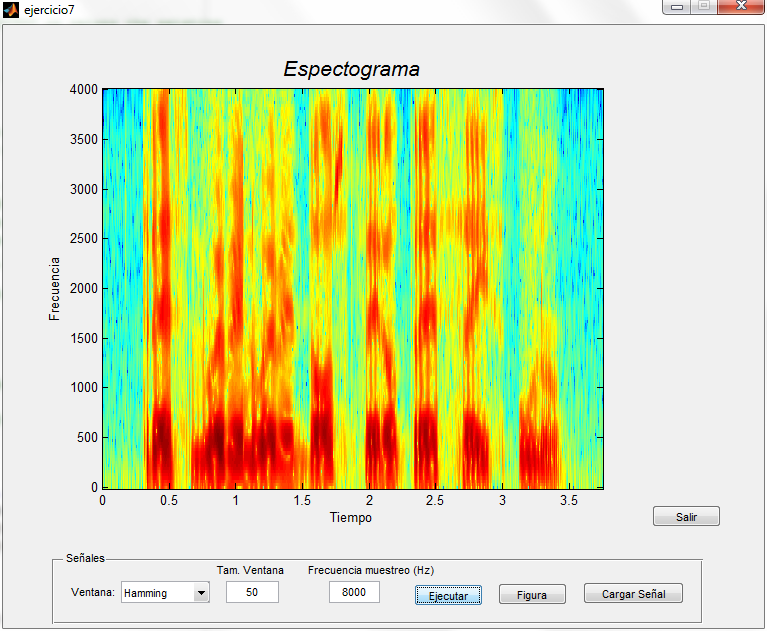
\includegraphics[scale=.8]{ej7-1.png}}\\
\hspace*{-.75in}{
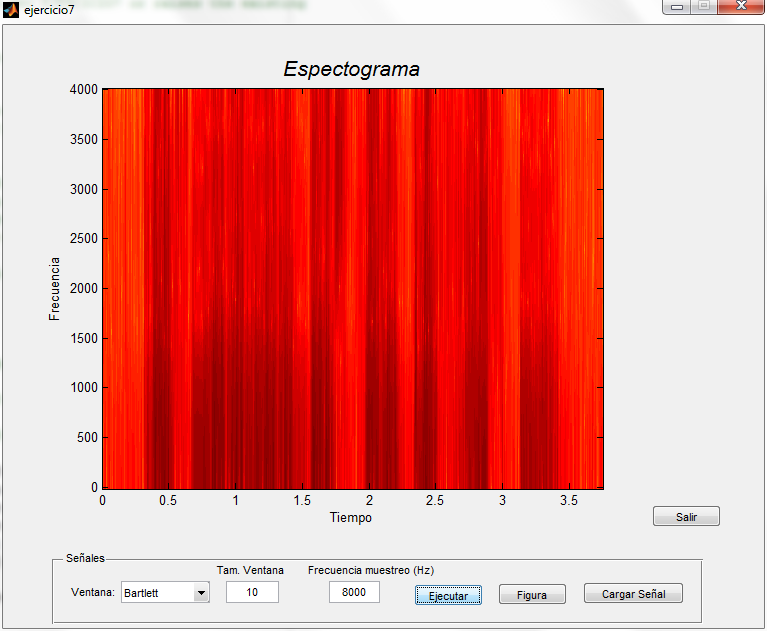
\includegraphics[scale=.8]{ej7-2.png}}\\
\hspace*{-.75in}{
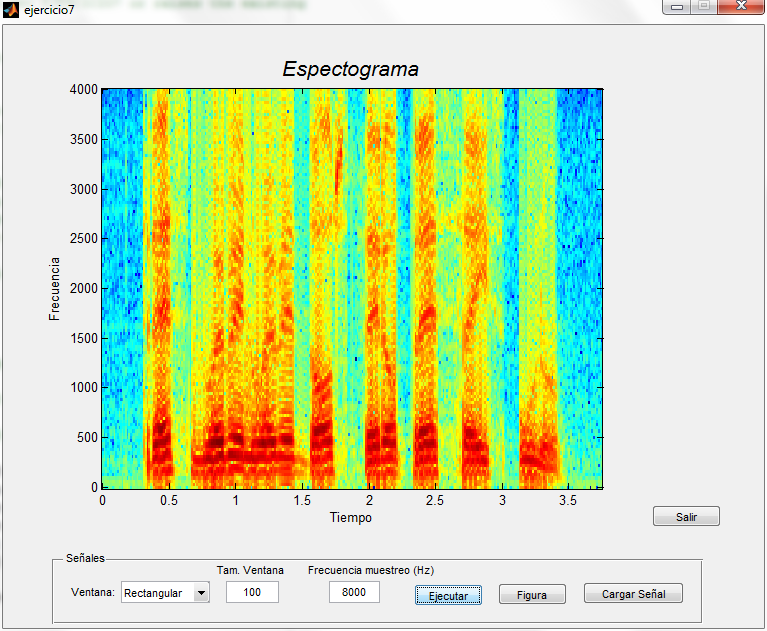
\includegraphics[scale=.8]{ej7-3.png}}\\

El funcionamiento de la interfaz es el siguiente:\\
\begin{itemize}
\item Para ejecutar dicha interfaz nos situamos en el directorio donde se encuentra y ejecutamos en la línea de comandos de matlab: ``ejercicio7''.
\item Pulsamos el botón de cargar señal y nos abrirá un gestor de ficheros en dónde podemos seleccionar el archivo de señal (asc) que deseemos.
\item Una vez cargado tendremos acceso a la ejecución del espectograma para un tipo de ventana que queramos, para un tamaño de la misma y una frecuencia de muestro expresada en Hz.
\item Pulsamos el botón ejecutar y nos saldrá en el recuadro para tal efecto nuestro espectograma.
\item Opcionalmente podemos abrir el resultado en una nueva ventana pulsando el botón ``Figura'' y así podremos observarla con más detenimiento.
\item Para salir de la interfaz podemos pulsar el botón ``Salir'' o cerrando simplemente la ventana.
\end{itemize}
\end{enumerate}
\end{document}

